\documentclass[tikz, border=3mm]{standalone}
\usepackage{tikz}
% Required libraries
\usetikzlibrary{
    arrows.meta,         % For arrow tips
    decorations.markings,% For placing arrows along paths
    calc,                % For coordinate calculations (e.g., midpoint)
    positioning          % For label positioning (optional but nice)
}

\begin{document}
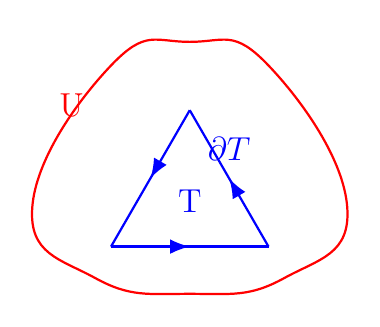
\begin{tikzpicture}[
    >=Latex, % Set default arrow tip style
    % Style for placing an arrow in the middle of a path segment
    midarrow/.style={
        decoration={markings, mark=at position 0.5 with {\arrow{Latex[length=2.5mm]}}}, % Adjust arrow size if needed
        postaction={decorate}
    }
]

    % Define Triangle Vertices (adjust coordinates for desired shape/position)
    \coordinate (A) at (0.5, 0.5);
    \coordinate (B) at (2.5, 0.5);
    \coordinate (C) at (1.5, {0.5+sqrt(3)}); % approx (1.5, 2.23) -> equilateral side 2

    % Draw the Outer Blob 'U'
    % Use 'plot smooth cycle' with estimated coordinates. Adjust as needed.
    \draw[red, thick] plot [smooth cycle, tension=0.8] coordinates {
        (0.3, 0.1)    % Below A
        (-0.5, 1.0)   % Left of A/C
        (0.5, 2.8)    % Above C left
        (1.5, 3.1)    % Topmost
        (2.5, 2.8)    % Above C right
        (3.5, 1.0)    % Right of B/C
        (2.7, 0.1)    % Below B
        (1.5, -0.1)   % Bottom middle
    };
    \node[red, font=\large] at (0, 2.3) {U}; % Label U near top-left

    % Draw the Triangle Edges (Boundary ∂T) with Counter-Clockwise Arrows
    \draw[blue, thick, midarrow] (A) -- (B); % A to B
    \draw[blue, thick, midarrow] (B) -- (C); % B to C
    \draw[blue, thick, midarrow] (C) -- (A); % C to A

    % Add Triangle Labels ('T' and '∂T')
    % Calculate centroid for T label (center of triangle)
    \coordinate (Centroid) at (barycentric cs:A=1,B=1,C=1);
    \node[blue, font=\large] at (Centroid) {T}; % Label T inside

    % Position ∂T near the midpoint of edge B--C, slightly outside
    \node[blue, font=\large, above=3pt] at ($(B)!0.5!(C)$) {$\partial T$};

\end{tikzpicture}
\end{document}